\section{SAME}
\label{sec:resultado_validacao_same}

\subsection{Calibração de Canal}
\label{sec:resultado_calibracao_canal_same}

Cada canal de medida da SAME converte a leitura do conversor
analógico-digital em grandeza física por uma reta: o valor medido é o produto
da tensão presente no pino do conversor por um coeficiente de escala, somado a
um deslocamento de zero. Os dois números saem do projeto da cadeia --- a
sensibilidade do sensor e a atenuação do divisor --- e ficam no arquivo de
configuração compartilhado entre o \textit{firmware} e a aplicação de
supervisão, de modo que as duas pontas do sistema interpretam a mesma leitura
da mesma forma.

No caminho de corrente, a sensibilidade adotada é a do sensor de efeito Hall
com o condutor passando uma única vez pelo furo do toróide,
\SI{18,750}{\milli\volt\per\ampere}, levantada na caracterização estática
(\autoref{sec:resultado_sensor_corrente}). A saída do sensor repousa em
\SI{2,5}{\volt} e chegaria a \SI{3,625}{\volt} em \SI{60}{\ampere}, acima dos
\SI{3,3}{\volt} que o conversor aceita; por isso ela passa por um divisor de
\SI{2,0}{\kilo\ohm} e \SI{18}{\kilo\ohm}, que atenua o sinal em
\num{0,900}. A cadeia completa fica com \SI{16,875}{\milli\volt\per\ampere},
o que corresponde a \SI{47,7}{\milli\ampere} por degrau do conversor. No
caminho de tensão, o divisor de \SI{130}{\kilo\ohm} e \SI{7,5}{\kilo\ohm}
atenua em \num{0,0545455} e estabelece fundo de escala de \SI{60,5}{\volt},
o dobro da tensão de barramento, com folga para o sobressinal de comutação;
o degrau resultante é de \SI{14,8}{\milli\volt}. A
\autoref{tab:resultado_calibracao_canal_same} reúne os dois caminhos.

\begin{table}[H]
    \centering
    \caption{Escala e resolução dos canais de medida da SAME}
    \label{tab:resultado_calibracao_canal_same}
    \begin{tabular}{lcccc}
        \toprule
        \textbf{Canal} & \textbf{Atenuação} & \textbf{Escala da cadeia} &
        \textbf{Degrau do ADC} & \textbf{Faixa válida} \\
        \midrule
        Corrente --- fases $A$, $B$ e $C$ & \num{0,900} &
        \SI{16,875}{\milli\volt\per\ampere} & \SI{47,7}{\milli\ampere} &
        $\pm\SI{70}{\ampere}$ \\
        Tensão --- fases $A$, $B$ e $C$ & \num{0,0545455} &
        \SI{54,5}{\milli\volt\per\volt} & \SI{14,8}{\milli\volt} &
        \SI{-1}{\volt} a \SI{65}{\volt} \\
        \bottomrule
    \end{tabular}

    \vspace{2pt}
    {\small Fonte: Autor (2026)}
\end{table}

A faixa válida da tabela não é folga de projeto: é critério de diagnóstico.
Leitura fora dela indica sensor saturado, cabo desconectado ou referência
aberta, e a placa a trata como falha em vez de dado.

O deslocamento de zero recebe tratamento diferente do coeficiente de escala.
O valor de projeto serve apenas como ponto de partida, porque o repouso do
sensor de corrente varia de peça para peça e com a temperatura. Nas três
configurações do ensaio de caracterização (\autoref{apendice:ensaio_hall}), a
leitura a corrente nula ficou em \SI{2,48570}{\volt}, \SI{2,48640}{\volt} e
\SI{2,49150}{\volt} --- \SI{5,8}{\milli\volt} de espalhamento, que nesta
cadeia equivalem a \SI{0,31}{\ampere} de corrente inexistente. O efeito é
mais grave do que o valor sugere: por ser comum às três fases, esse erro
atravessa a transformada de Clarke como componente de sequência zero e
aparece na estimativa de força contraeletromotriz do observador como sinal
espúrio. Por isso o \textit{firmware} mede o repouso real a cada
energização, com o ESC parado, e sobrescreve o valor de projeto antes de
iniciar a aquisição.

Cabe uma ressalva sobre o alcance dessa verificação. Nos ensaios com o motor
girando (\autoref{sec:resultado_setup_scope}), as tensões de fase foram
medidas diretamente pelas pontas do osciloscópio, sem passar pelo divisor da
placa; as correntes, sim, vieram dos sensores da SAME. A cadeia de corrente
foi, portanto, exercitada com o motor em operação, enquanto a de tensão
permanece verificada apenas pelo projeto do divisor. As formas de onda reais
de tensão e corrente adquiridas com o motor girando são as apresentadas na
\autoref{fig:bancada_smo_alfabeta}.

\subsection{Sensor de Corrente}
\label{sec:resultado_sensor_corrente}

O conjunto núcleo toroidal com sensor Hall foi caracterizado pelo
procedimento da \autoref{sec:same_sensor_corrente}, nas três configurações de
enrolamento previstas. A \autoref{fig:hall_vout_i} apresenta a tensão de saída
em função da corrente imposta, com as retas ajustadas por mínimos quadrados; a
coleta completa está no Apêndice~\ref{apendice:ensaio_hall}. A
\autoref{fig:ensaio_hall_foto} mostra a montagem utilizada.

\begin{figure}[H]
    \centering
    \caption{Montagem do ensaio de caracterização do conjunto núcleo--sensor}
    \label{fig:ensaio_hall_foto}
    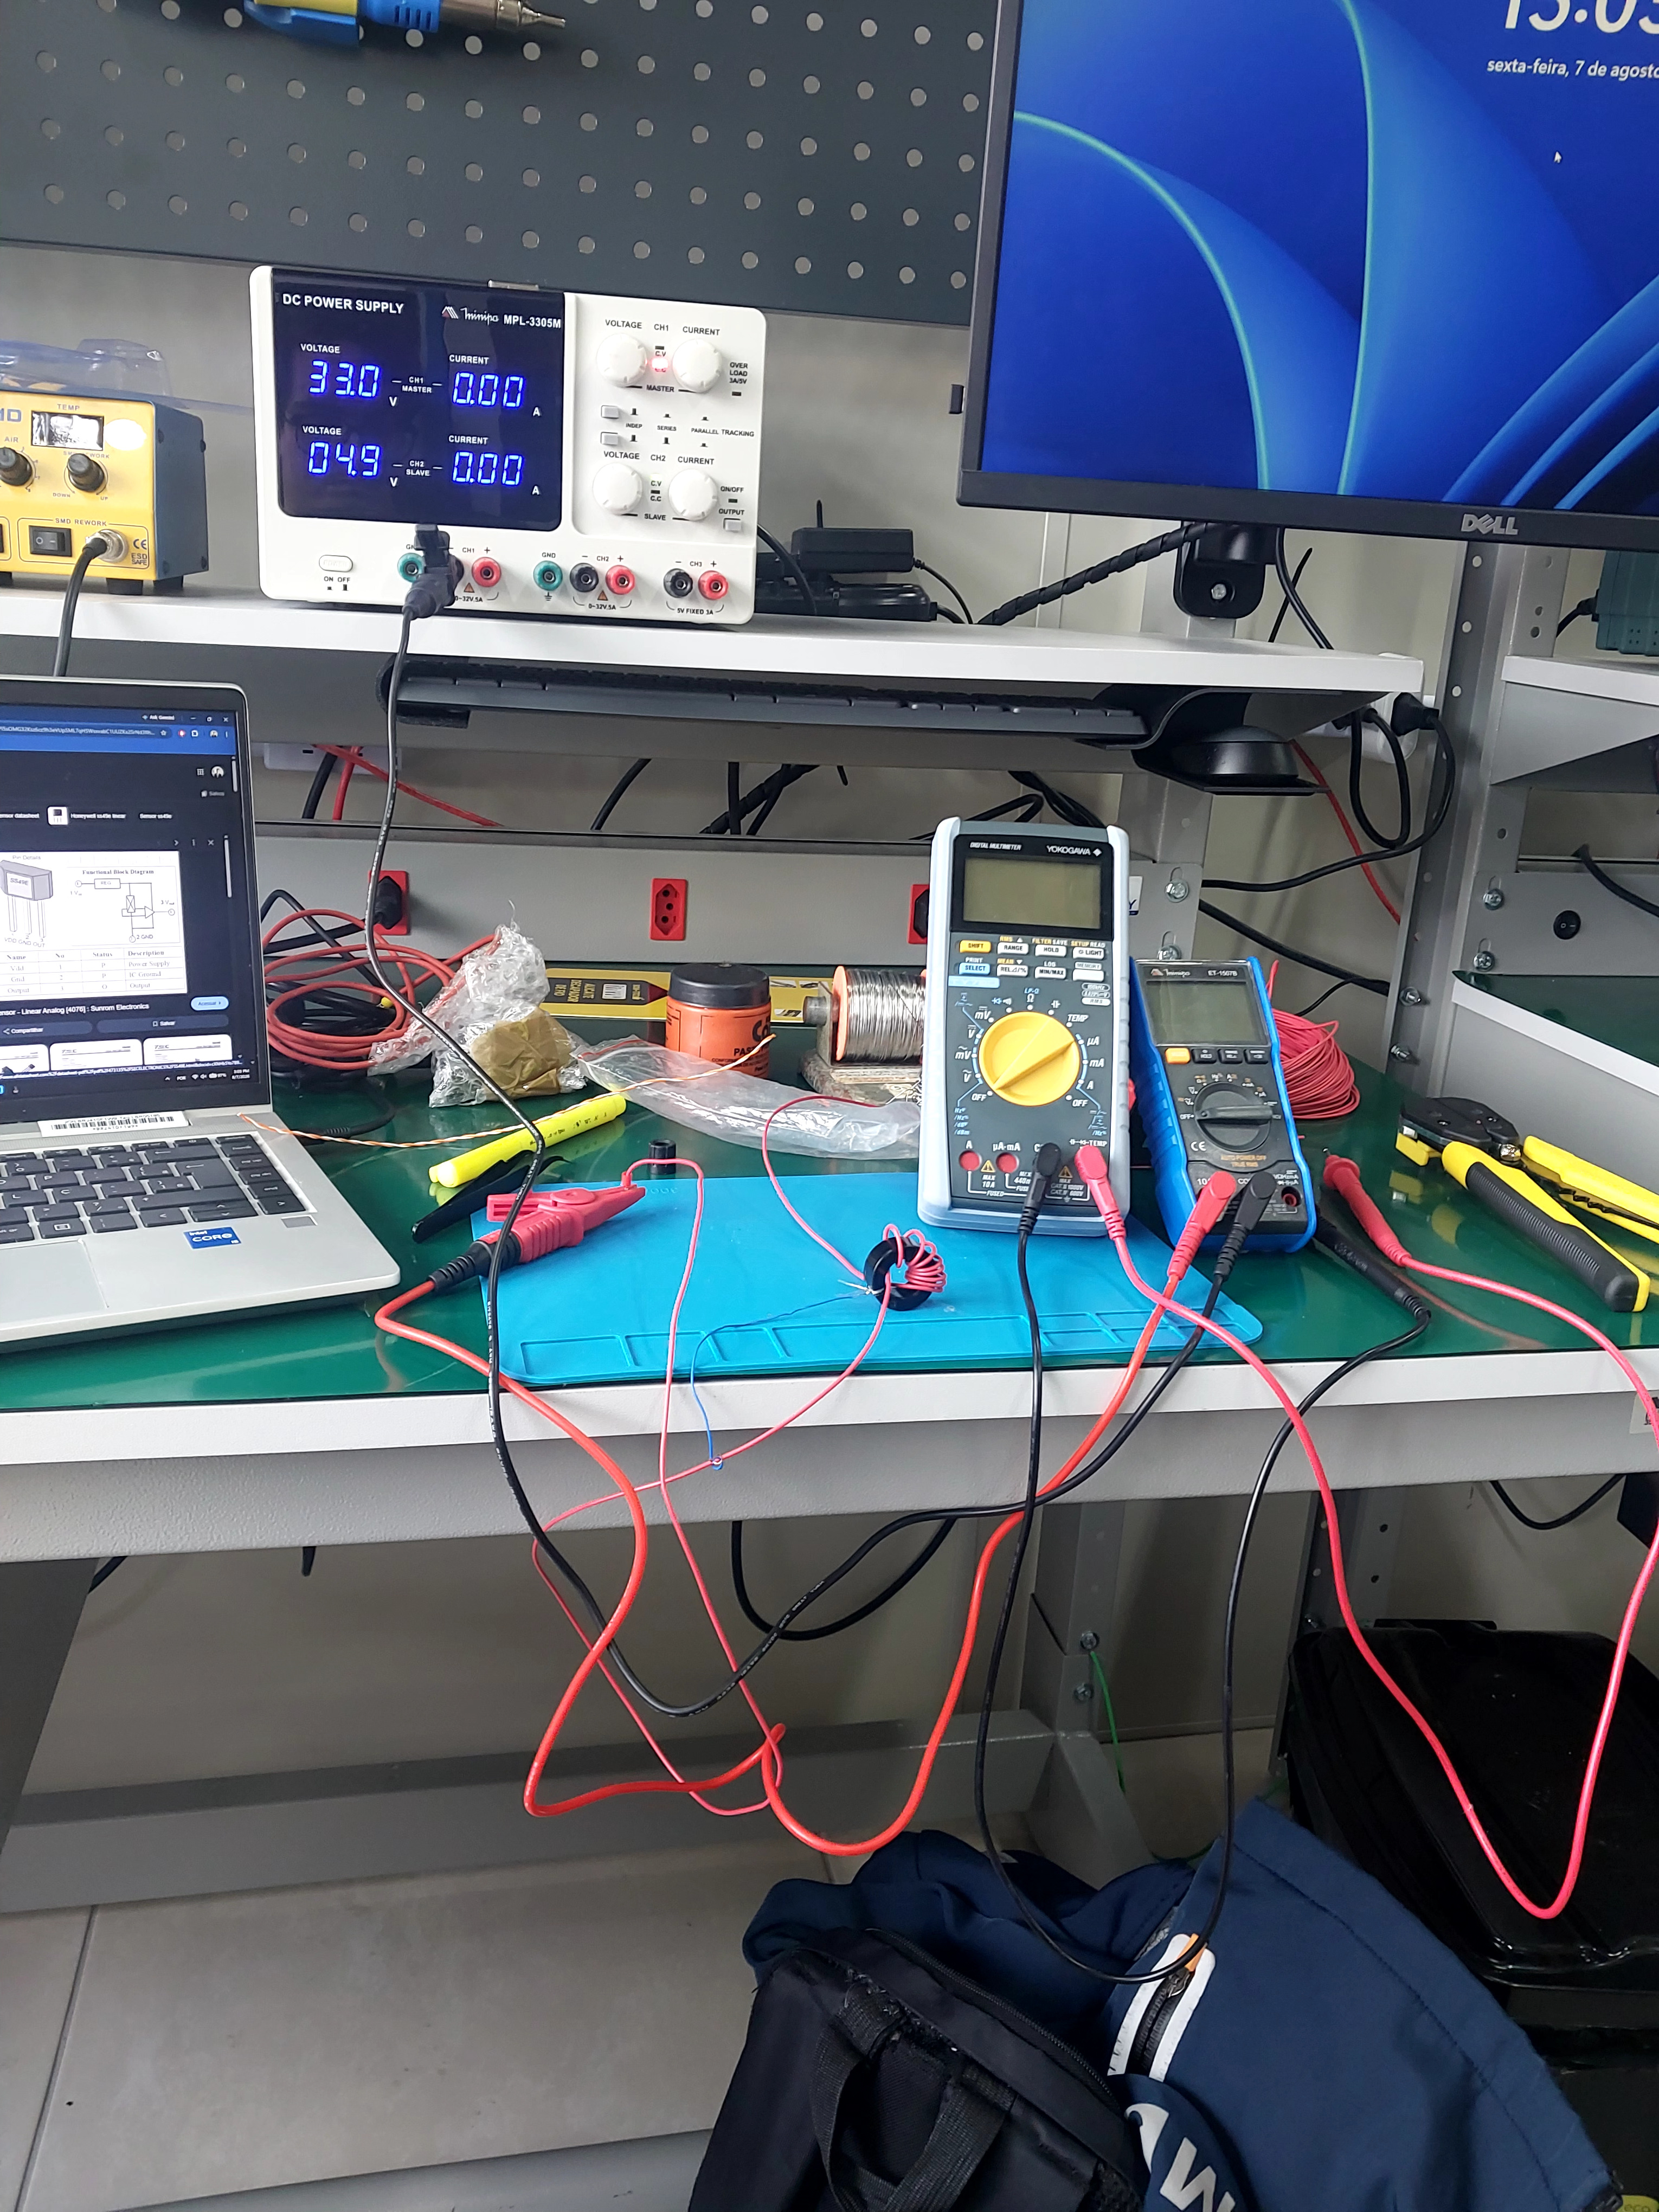
\includegraphics[width=0.5\linewidth]{Textuais/Imgs/Resultados/ensaio_sensor_corrente.jpg}

    Fonte: Autor (2026)
\end{figure}

\begin{figure}[H]
    \centering
    \caption{Tensão de saída do SS49E em função da corrente imposta}
    \label{fig:hall_vout_i}
    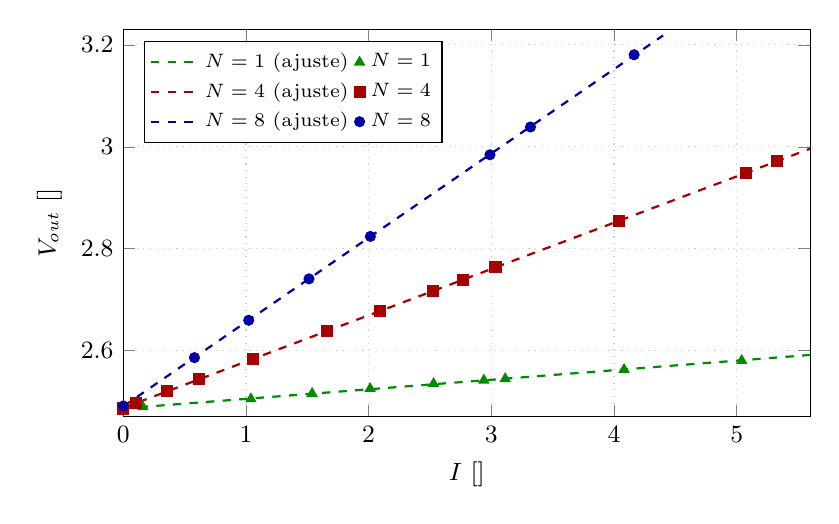
\begin{tikzpicture}
        \begin{axis}[
            width=0.85\textwidth, height=6.5cm,
            xlabel={$I$ [\si{\ampere}]}, ylabel={$V_{out}$ [\si{\volt}]},
            xmin=0, xmax=5.6, ymin=2.47, ymax=3.23,
            grid=both, grid style={dotted,gray!40},
            legend pos=north west,
            legend style={font=\scriptsize, inner sep=2pt},
            legend columns=2,
            tick label style={font=\small}, label style={font=\small},
        ]
            \addplot[dashed, green!55!black, thick, domain=0:5.6] {0.018750*x + 2.486645};
            \addlegendentry{$N=1$ (ajuste)}
            \addplot[only marks, mark=triangle*, mark size=2pt, green!55!black]
                coordinates {
                    (0.000,2.48570)(0.159,2.48975)(1.040,2.50530)(1.539,2.51590)
                    (2.012,2.52550)(2.529,2.53520)(2.939,2.54200)
                    (3.113,2.54490)(4.082,2.56270)(5.041,2.58050)};
            \addlegendentry{$N=1$}
            \addplot[dashed, red!65!black, thick, domain=0:5.6] {0.090866*x + 2.487632};
            \addlegendentry{$N=4$ (ajuste)}
            \addplot[only marks, mark=square*, mark size=2pt, red!65!black]
                coordinates {
                    (0.000,2.48640)(0.101,2.49780)(0.355,2.52050)(0.620,2.54420)
                    (1.056,2.58320)(1.662,2.63800)(2.094,2.67800)
                    (2.522,2.71710)(2.766,2.73900)(3.034,2.76340)
                    (4.038,2.85450)(5.077,2.94880)(5.329,2.97200)};
            \addlegendentry{$N=4$}
            \addplot[dashed, blue!65!black, thick, domain=0:4.4] {0.165417*x + 2.490699};
            \addlegendentry{$N=8$ (ajuste)}
            \addplot[only marks, mark=*, mark size=1.8pt, blue!65!black]
                coordinates {
                    (0.000,2.49150)(0.580,2.58630)(1.022,2.65960)(1.514,2.74090)
                    (2.014,2.82410)(2.989,2.98440)(3.319,3.03893)
                    (4.164,3.18070)};
            \addlegendentry{$N=8$}
        \end{axis}
    \end{tikzpicture}

    Fonte: Autor (2026)
\end{figure}

Convertendo a corrente em densidade de fluxo pela
\autoref{eq:B_hopkinson}, as três configurações passam a ocupar um mesmo eixo
e podem ser confrontadas entre si e contra a sensibilidade típica de catálogo,
como mostra a \autoref{fig:hall_dv_b}. O ensaio com oito espiras estende a
varredura até \SI{516}{\gauss}, contra \SI{78}{\gauss} da configuração de uso
real, o que permite verificar a linearidade em mais da metade da faixa
magnética do elemento.

\begin{figure}[H]
    \centering
    \caption{Curva de transferência $\Delta V \times B$ das três configurações}
    \label{fig:hall_dv_b}
    \begin{tikzpicture}
        \begin{axis}[
            width=0.85\textwidth, height=6.5cm,
            xlabel={$B$ [G]}, ylabel={$\Delta V$ [\si{\milli\volt}]},
            xmin=0, xmax=540, ymin=0, ymax=760,
            grid=both, grid style={dotted,gray!40},
            legend pos=north west,
            legend style={font=\scriptsize, inner sep=2pt},
            tick label style={font=\small}, label style={font=\small},
        ]
            \addplot[dotted, black, very thick, domain=0:540] {1.4*x};
            \addlegendentry{Típico de catálogo (\SI[per-mode=symbol]{1,40}{\milli\volt\per\gauss})}
            \addplot[only marks, mark=triangle*, mark size=2pt, green!55!black]
                coordinates {
                    (0.00,-0.945)(2.47,3.105)(16.12,18.655)(23.86,29.255)
                    (31.19,38.855)(39.21,48.555)(45.57,55.355)
                    (48.26,58.255)(63.29,76.055)(78.16,93.855)};
            \addlegendentry{$N=1$ --- \SI[per-mode=symbol]{1,209}{\milli\volt\per\gauss}}
            \addplot[only marks, mark=square*, mark size=2pt, red!65!black]
                coordinates {
                    (0.00,-1.232)(6.26,10.168)(22.02,32.868)(38.45,56.568)
                    (65.49,95.568)(103.07,150.368)(129.86,190.368)
                    (156.40,229.468)(171.53,251.368)(188.16,275.768)
                    (250.42,366.868)(314.85,461.168)(330.48,484.368)};
            \addlegendentry{$N=4$ --- \SI[per-mode=symbol]{1,465}{\milli\volt\per\gauss}}
            \addplot[only marks, mark=*, mark size=1.8pt, blue!65!black]
                coordinates {
                    (0.00,0.801)(71.94,95.601)(126.76,168.901)(187.78,250.201)
                    (249.80,333.401)(370.73,493.701)(411.66,548.231)
                    (516.47,690.001)};
            \addlegendentry{$N=8$ --- \SI[per-mode=symbol]{1,334}{\milli\volt\per\gauss}}
        \end{axis}
    \end{tikzpicture}

    Fonte: Autor (2026)
\end{figure}

Os resíduos do ajuste linear (\autoref{fig:hall_res}) permanecem abaixo de
\SI{1,24}{\milli\volt} nas três configurações, sem estrutura de curvatura que
denuncie saturação do ferrite ou compressão do elemento Hall no extremo da
faixa varrida. Referido ao \textit{span} completo do elemento --- os
\SI{2,8}{\volt} correspondentes a $\pm\SI{1000}{\gauss}$ com a sensibilidade
medida ---, esse desvio equivale a \SI{0,04}{\percent}, muito abaixo da
linearidade de $-\SI{0,7}{\percent}$ do \textit{span} especificada em
catálogo.

\begin{figure}[H]
    \centering
    \caption{Resíduos do ajuste linear por configuração de enrolamento}
    \label{fig:hall_res}
    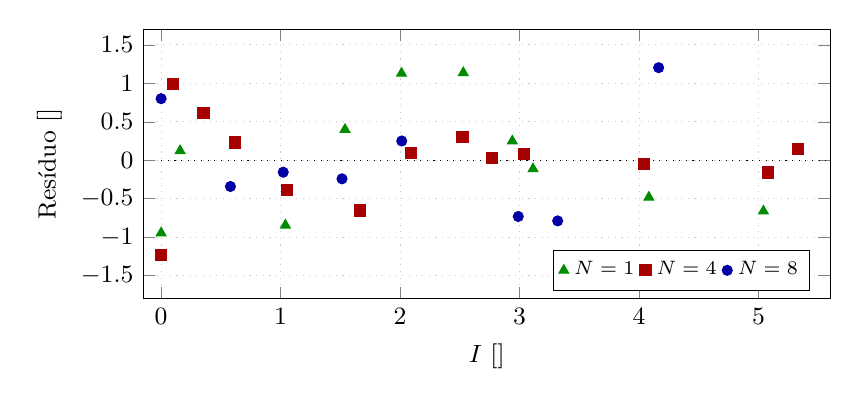
\begin{tikzpicture}
        \begin{axis}[
            width=0.85\textwidth, height=5cm,
            xlabel={$I$ [\si{\ampere}]}, ylabel={Resíduo [\si{\milli\volt}]},
            xmin=-0.15, xmax=5.6, ymin=-1.8, ymax=1.7,
            ytick={-1.5,-1,-0.5,0,0.5,1,1.5},
            grid=both, grid style={dotted,gray!40},
            legend pos=south east,
            legend style={font=\scriptsize, inner sep=2pt},
            legend columns=3,
            tick label style={font=\small}, label style={font=\small},
        ]
            \addplot[dotted, black, domain=0:5.6, forget plot] {0};
            \addplot[only marks, mark=triangle*, mark size=2pt, green!55!black]
                coordinates {
                    (0.000,-0.945)(0.159,0.124)(1.040,-0.844)(1.539,0.400)
                    (2.012,1.131)(2.529,1.138)(2.939,0.250)
                    (3.113,-0.112)(4.082,-0.481)(5.041,-0.661)};
            \addlegendentry{$N=1$}
            \addplot[only marks, mark=square*, mark size=2pt, red!65!black]
                coordinates {
                    (0.000,-1.232)(0.101,0.990)(0.355,0.610)(0.620,0.231)
                    (1.056,-0.387)(1.662,-0.652)(2.094,0.094)
                    (2.522,0.303)(2.766,0.032)(3.034,0.080)
                    (4.038,-0.050)(5.077,-0.160)(5.329,0.142)};
            \addlegendentry{$N=4$}
            \addplot[only marks, mark=*, mark size=1.8pt, blue!65!black]
                coordinates {
                    (0.000,0.801)(0.580,-0.341)(1.022,-0.155)(1.514,-0.241)
                    (2.014,0.251)(2.989,-0.731)(3.319,-0.788)
                    (4.164,1.204)};
            \addlegendentry{$N=8$}
        \end{axis}
    \end{tikzpicture}

    Fonte: Autor (2026)
\end{figure}

A \autoref{tab:hall_result} reúne os parâmetros extraídos de cada
configuração. A coluna $S$ é o coeficiente angular medido, em milivolts por
ampere de corrente no primário; a coluna $S_H$ é a sensibilidade do elemento
Hall obtida dividindo $S$ pelo gradiente $N\,\mathrm{d}B/\mathrm{d}I$ da
\autoref{eq:dBdI}, e é a grandeza diretamente comparável ao
\textit{datasheet}.

\begin{table}[H]
    \centering
    \caption{Parâmetros do conjunto núcleo--sensor por configuração de enrolamento}
    \label{tab:hall_result}
    \begin{tabular}{cccccc}
        \toprule
        \textbf{$N$} & \textbf{$B$ varrido [G]} & \textbf{$S$ [\si{\milli\volt\per\ampere}]} &
        \textbf{$S_H$ [\si{\milli\volt\per\gauss}]} & \textbf{Desvio do típico} & \textbf{$R^2$} \\
        \midrule
        1 & 0 -- 78  & 18{,}75 $\pm$ 0{,}16  & 1{,}209 & $-13{,}6\%$ & 0{,}99939 \\
        4 & 0 -- 330 & 90{,}87 $\pm$ 0{,}09  & 1{,}465 & $+4{,}7\%$  & 0{,}99999 \\
        8 & 0 -- 516 & 165{,}42 $\pm$ 0{,}20 & 1{,}334 & $-4{,}7\%$  & 0{,}99999 \\
        \midrule
        \multicolumn{3}{l}{Média das três configurações} & 1{,}336 & $-4{,}6\%$ & -- \\
        \multicolumn{3}{l}{Típico de catálogo} & 1{,}400 & -- & -- \\
        \bottomrule
    \end{tabular}

    \vspace{2pt}
    {\small Fonte: Autor (2026)}
\end{table}

As três configurações resultam em sensibilidade dentro da faixa especificada
pelo fabricante (\SIrange{1,00}{1,75}{\milli\volt\per\gauss}), com média de
\SI{1,336}{\milli\volt\per\gauss} --- desvio de $-\SI{4,6}{\percent}$ frente
ao típico. A tensão de repouso medida, entre \SI{2,487}{\volt} e
\SI{2,491}{\volt} nas três coletas, também se enquadra na faixa de catálogo
(\SIrange{2,25}{2,75}{\volt}).

O ponto que exige leitura cuidadosa é a dispersão de $S_H$ entre as
configurações: \SI{1,209}{}, \SI{1,465}{} e
\SI{1,334}{\milli\volt\per\gauss}, ou seja $\pm\SI{9,6}{\percent}$ em torno da
média, sem tendência monotônica com $N$. Como se trata de uma única unidade
física de sensor, $S_H$ é uma propriedade fixa e não pode variar de um ensaio
para o outro; a dispersão observada não está no elemento Hall, e sim na
hipótese de que $B$ é estritamente proporcional a $N\,I$ com o fator
$A_l/A_e$ de catálogo. Isso é coerente com as duas fontes de erro que essa
hipótese carrega: a tolerância de $\pm\SI{15}{\percent}$ do próprio $A_l$ e a
diferença de acoplamento entre uma espira única atravessando o furo e um
enrolamento distribuído externamente ao toróide, que fecha um caminho de fluxo
de dispersão distinto. A qualidade do ajuste dentro de cada configuração
($R^2 \geq 0{,}9994$) confirma que a dispersão é sistemática entre montagens,
não ruído de medição.

A consequência prática é que o artifício de $N$ espiras é válido para verificar
a linearidade e situar o sensor na faixa de catálogo --- o que foi feito ---
mas não substitui a calibração na topologia de uso. O ganho do sensor adotado
para o projeto é o da configuração $N = 1$,
\SI{18,75}{\milli\volt\per\ampere} --- valor sobre o qual o estágio de
condicionamento do caminho de corrente foi dimensionado
(\autoref{sec:same_sensor_corrente}), já que a saída do sensor, centrada em
\SI{2,5}{\volt}, não pode ser levada direto ao ADC de \SI{3,3}{\volt}.
